\lab{Algorithms}{Speech Recognition}{Speech Recognition}
\objective{Understand how speech recognition via CDHMMs works, and implement a simplified speech recognition system.}

Hidden Markov Models are the basis of modern speech recognition systems. We assume that a short speech signal can be viewed as a stationary signal, and so we can divide a speech signal into small frames (approximately $30$ ms or so). We can take this framed signal and through a series of transformations represent it by mel-frequency cepstral coefficients (MFCCs), keeping only the first $K$ (say $K = 10$). Viewing these MFCCs as continuous observations in $\mathbb{R}^{K}$, we can train a GMMHMM on sequences of MFCCs for a given word, spoken multiple times. Doing this for several words, we have a collection of GMMHMMs, one for each word. Given a new speech signal, after framing and decomposing it into its MFCC array, we can score the signal against each GMMHMM, returning the word whose GMMHMM scored the highest.

In practice, a GMMHMM is not trained for each word in a vocabulary (that would be ludicrous for a large vocabulary), but rather on \emph{phonemes}, or distinct sounds. The English language has $44$ phonemes, yielding $44$ different GMMHMMs. By correctly classifying a signal by its phonemes, we can determine what word was spoken. Doing so is beyond the scope of this program, so we will simply train GMMHMMs on five words/phrases: biology, mathematics, political science, psychology, and statistics.

In a Linux environment, plug in your USB microphone headset and in the command line, enter
\texttt{arecord -l}
Note under which card the USB audio device is listed, as well as the device number. This will likely be card 1, device 0.

To record audio from the command line and save it as \texttt{test.wav} in your current working directory, enter
\texttt{arecord -f S16\_LE --rate=44100 -D hw:1,0 -d 2 test.wav}
This will record the audio from your USB microphone for $2$ seconds, sampling at a rate of $44100$ samples per second, saving the samples as signed $16$-bit numbers at the file name \texttt{test.wav}. We can read the wav file into python with the \li{scipy.io.wavfile} module:
\begin{lstlisting}
: import numpy as np
: import scipy.io.wavfile as wavfile
: sample = wavfile.read("test.wav")[1]
\end{lstlisting}

The object \li{sample} will be a vector of integers of length $88200 = 44100*2$. This in and of itself is not very useful. We must transform the data in a series of steps before it will be useful. We must first break the sample into \emph{frames}, each of some small length ($30$ ms). We will overlap these frames to smooth out these cutoff areas. In short, each frame will overlap with the previous by $20$ ms. Doing so with a $2$ second sample yields $198$ frames, each frame containing $1323$ values from the original sample, overlapping $882$ values with each sample immediately preceding and following it. We let $f_{n}$ denote the $n^{\text{th}}$ entry of the frame $f$.

Because we have overlapped the samples, the most significant part of a frame is the middle $441$ entries. We decrease the effects of the edges of the frame by applying a window function, making the edges nearly zero, while keeping the middle large. We use the Hamming window, defined as 
\begin{equation*}
w(n) = 0.54 - 0.46 \cos \left( \frac{2\pi (n + 0.5)}{N} \right)
\end{equation*}
where $N = 1323$ is the length of the frame. We window each frame, computing $\tilde{f}_{n} = f_{n}w(n)$.

After windowing each frame, we then apply a filtering process known as \emph{preemphasis} used to improve the signal-to-noise ratio as follows:
\begin{equation*}
\widehat{f}_{n} = \tilde{f}_{n} - 0.95 \tilde{f}_{n-1}
\end{equation*}

We must next perform the discrete fourier transform of each frame, though to get a more refined view of the frequency spectrum, we must pad our vector with zeros to make it of length $2048$. We also will only keep approximately half of the returned vector, then take the square of the magnitude of each complex component.

We will ultimately be taking the logarithm of this transformed frame, so we must make sure all entries are slightly positive. We must then transform this into the \emph{mel scale}, which is a scale of pitches which listeners tend to judge to be of equal distance from one another. We make this transformation by binning the frames into $40$ bins, according to the overlapping triangular binning scheme in Figure \ref{fig:binning}.

\begin{figure}
\centering
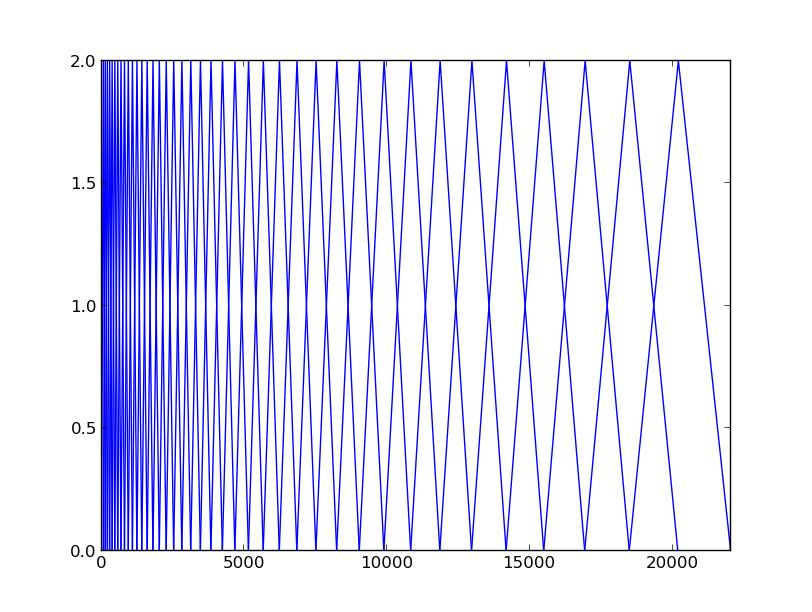
\includegraphics[width=\textwidth]{melfilterbank.jpeg}
\caption{Binning scheme to transform linearly spaced frequency to mel scale.}
\label{fig:binning}
\end{figure}

If we want $40$ bins where the length of our padded frames is $2048$, then we can compute a \emph{mel filter bank} $M$ which is a matrix used to bin our transformed frame into the mel scale. We can now bin our frame by multiplying this matrix against the transformed frame. We also take the logarithm of the binned values, after which we compute the discrete cosine transform (DCT) of the returned values via a DCT transformation matrix, and then finally truncate to only keep ten values, called the mel frequency cepstral coefficients (MFCC). Note that we do not typically keep the first MFCC.

Normally we do this for all desired frames, storing each vector of MFCCs as a row in an array, after which we normalize by subtracting the mean of the MFCC rows, and divide by the standard deviations. We have provided you with code that allows you to compute these MFCCs quickly:
\begin{lstlisting}
: import MFCC
: mfccs = MFCC.extract(sample)
\end{lstlisting}

\begin{problem}
Record the word \emph{mathematics} as a $2$ second WAV file $20$ times, and decompose each file into its MFCC array, storing these in a list. Do this also for the words/phrases \emph{biology}, \emph{political science}, \emph{psychology}, and \emph{statistics}. Be sure you complete each word/phrase in the $2$ second window.
\end{problem}

For a specific word, given enough samples of that word decomposed into its MFCCs, we can train a GMMHMM. For this, we will use the file \li{gmmhmm.py} provided, as this is a stable implementation of GMMHMM algorithms. To facilitate random restarts, we need a function to provide initializations for the initial state distribution and the transition matrix.

\begin{problem}
Write a function that initializes the initial state distribution and transition matrix for a GMMHMM with $n$ states. You may have done this in a previous lab, so feel free to copy and paste.
\end{problem}

Let \li{samples} be a list of arrays, where each row in each array is a set of MFCCs corresponding to a frame in a sample for a given word. Using a function \li{initialize()} that returns a random initial state distribution and transition matrix, we will show how to train a GMMHMM with $5$ states, each having an output distribution as a GMM with $3$ mixture components. We also look at the log-likelihood of the data, given the trained model.
\begin{lstlisting}
: import gmmhmm
: startprob, transmat = initialize(5)
: model = gmmhmm.GMMHMM(n_components=5, n_mix=3, transmat=transmat, startprob=startprob, cvtype='diag')
: model.covars_prior = 0.01
: model.fit(samples, init_params='mc', var=0.1)
: print model.logprob
\end{lstlisting}

\begin{problem}
Train a GMMHMM on each of the words you previously recorded with at least $10$ random restarts, keeping the best model for each word. You might want to do this in parallel to save time.
\end{problem}

Given a trained model, we would like to compute the log-likelihood of a new sample. Letting \li{obs} be an array, each row of which is a set of MFCCs for a frame in a sample, we do this as follows:
\begin{lstlisting}
: score = model.score(obs)
\end{lstlisting}

\begin{problem}
Write a function that records a sample, converts it into its MFCC array, and then scores it on each of the five trained models. Return the word corresponding to the highest scoring model. Test your speech recognition system on each of the five words multiple times. How does it perform?
\end{problem}